\documentclass[12pt,a4paper,portuguese]{article}
\usepackage[T1]{fontenc}
\usepackage{babel}
\usepackage{graphicx}
\usepackage{float}
\title{Lista 1 - Analise Series temporais em oceano}
\author{Lucas Salimene}
\date{}

\begin{document}
	
	\maketitle
	\newpage
	
	\textbf{Parte I – Visualização e edição dos dados oceanográficos}
	
	

\begin{figure}[H]
	\centering
	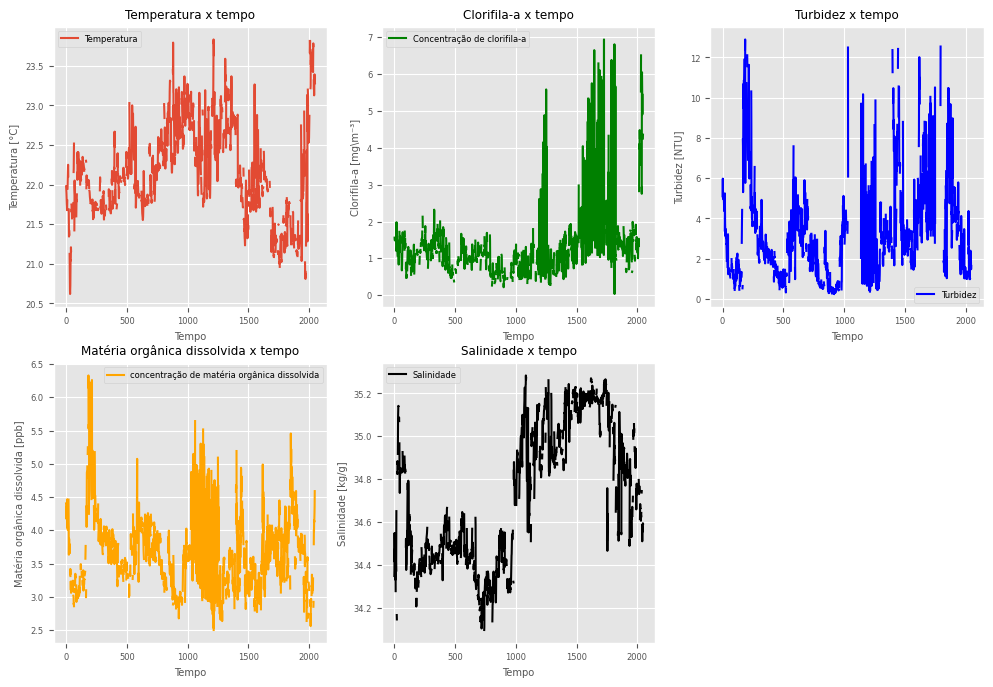
\includegraphics[width=1\linewidth]{lista1-1b}
	\caption{Variáveis disponível no dado do SIMCOSTA}
	\label{fig:lista1-1b}
\end{figure}
	Conforme se observa na figura \ref{fig:lista1-1b}, existe a necessidade de interpolação dos dados, pois existem lacunas nos mesmos.
	
\begin{figure}[H]
	\centering
	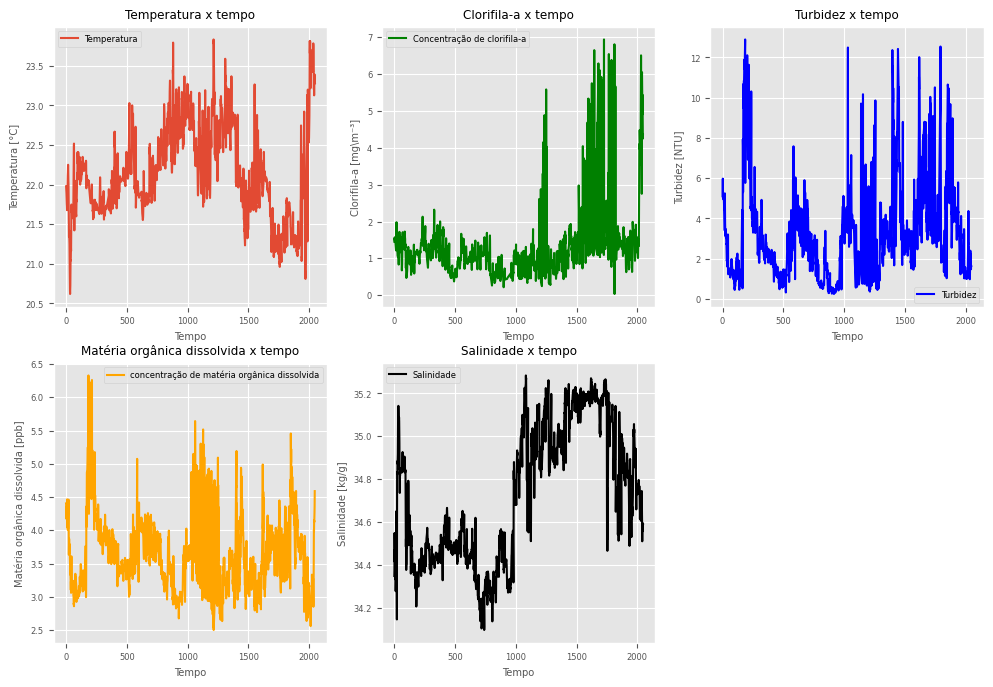
\includegraphics[width=1\linewidth]{lista1-1c}
	\caption{Variáveis disponível no dado do SIMCOSTA após interpolação linear}
	\label{fig:lista1-1c}
\end{figure}
	A figura \ref{fig:lista1-1c} mostra os dados após uma interpolação linear utilizando o pacote pandas do Python.
	\begin{verbatim}
pandas.DataFrame.interpolate
	\end{verbatim}
	É notável que mesmo após a interpolação os dados apresentam pontos que não representam o comportamento da série e podem ter ocorrido devido a algum erro/processo que não seja do interesse. Com isso surge a necessidade da utilização de uma edição na série temporal
	
	
\end{document}